\documentclass[12pt]{article}

\usepackage[a4paper,margin=1in]{geometry}
\usepackage{amsmath,amssymb,amsthm}
\usepackage{tikz}
\usepackage{enumitem}
\usepackage{array}

\setlength{\parindent}{0pt}
\setlength{\parskip}{0.75em}

\newtheorem{definition}{Definition}
\newtheorem{remark}{Remark}
\newtheorem{example}{Example}
\newtheorem{proposition}{Proposition}

\title{Lecture 13: Generalized Poisson Queue Models}
\author{MA4034 -- Time Series and Stochastic Processes}
\date{}

\begin{document}

\maketitle

\section{Generalized Poisson Model for a Queue}

In queueing theory, we are often interested in the probability that the system contains \(n\) customers in the long run.

Let
\[
p_n=P(\text{there are }n\text{ customers in the system at steady state}).
\]

The goal is to find
\[
p_0,p_1,p_2,\ldots
\]

In a generalized birth-death queue:

\begin{itemize}
    \item arrivals increase the system size,
    \item departures decrease the system size.
\end{itemize}

The arrival rate may depend on the current system size:
\[
\lambda_n=\text{arrival rate when there are }n\text{ customers}.
\]

The departure rate may also depend on the current system size:
\[
\mu_n=\text{departure rate when there are }n\text{ customers}.
\]

\begin{center}
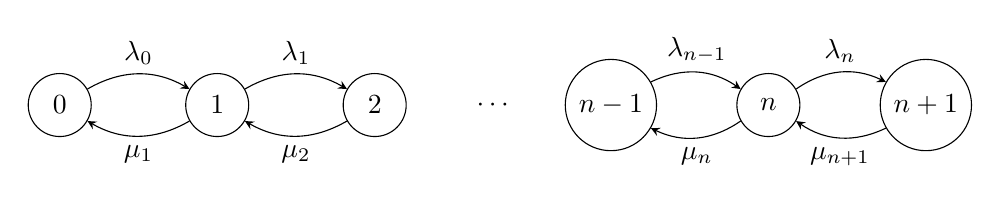
\begin{tikzpicture}[>=stealth, node distance=1.8cm]
    \node[circle,draw,minimum size=0.8cm] (0) at (0,0) {0};
    \node[circle,draw,minimum size=0.8cm] (1) at (2,0) {1};
    \node[circle,draw,minimum size=0.8cm] (2) at (4,0) {2};
    \node (dots1) at (5.5,0) {\(\cdots\)};
    \node[circle,draw,minimum size=0.8cm] (n1) at (7,0) {\(n-1\)};
    \node[circle,draw,minimum size=0.8cm] (n) at (9,0) {\(n\)};
    \node[circle,draw,minimum size=0.8cm] (np1) at (11,0) {\(n+1\)};

    \draw[->,bend left] (0) to node[above] {\(\lambda_0\)} (1);
    \draw[->,bend left] (1) to node[below] {\(\mu_1\)} (0);

    \draw[->,bend left] (1) to node[above] {\(\lambda_1\)} (2);
    \draw[->,bend left] (2) to node[below] {\(\mu_2\)} (1);

    \draw[->,bend left] (n1) to node[above] {\(\lambda_{n-1}\)} (n);
    \draw[->,bend left] (n) to node[below] {\(\mu_n\)} (n1);

    \draw[->,bend left] (n) to node[above] {\(\lambda_n\)} (np1);
    \draw[->,bend left] (np1) to node[below] {\(\mu_{n+1}\)} (n);
\end{tikzpicture}
\end{center}

This is called a birth-death process because the state can move only one step up or one step down.

\[
n\to n+1 \quad \text{arrival or birth},
\]
\[
n\to n-1 \quad \text{departure or death}.
\]

\section{Steady-State Balance Idea}

At steady state, the expected rate of flow into each state must equal the expected rate of flow out of that state.

For \(n>0\), state \(n\) can be entered in two ways:

\begin{itemize}
    \item from state \(n-1\) by an arrival,
    \item from state \(n+1\) by a departure.
\end{itemize}

So the expected rate of flow into state \(n\) is
\[
\lambda_{n-1}p_{n-1}+\mu_{n+1}p_{n+1}.
\]

State \(n\) can be left in two ways:

\begin{itemize}
    \item from state \(n\) to \(n+1\) by an arrival,
    \item from state \(n\) to \(n-1\) by a departure.
\end{itemize}

So the expected rate of flow out of state \(n\) is
\[
(\lambda_n+\mu_n)p_n.
\]

At equilibrium:
\[
\boxed{
\lambda_{n-1}p_{n-1}+\mu_{n+1}p_{n+1}
=
(\lambda_n+\mu_n)p_n,\qquad n=1,2,\ldots
}
\]

\section{Local Balance Equations}

For birth-death queues, we can usually use the simpler local balance equations:

\[
\boxed{
\lambda_{n-1}p_{n-1}=\mu_np_n,\qquad n=1,2,\ldots
}
\]

This says:

\begin{center}
flow from \(n-1\) to \(n\) equals flow from \(n\) back to \(n-1\).
\end{center}

For \(n=0\), the only neighboring state is 1. So:
\[
\lambda_0p_0=\mu_1p_1.
\]

Hence,
\[
p_1=\frac{\lambda_0}{\mu_1}p_0.
\]

For \(n=2\):
\[
\lambda_1p_1=\mu_2p_2.
\]

Substitute \(p_1\):
\[
p_2
=
\frac{\lambda_1}{\mu_2}p_1
=
\frac{\lambda_1}{\mu_2}\frac{\lambda_0}{\mu_1}p_0.
\]

So
\[
p_2=\frac{\lambda_1\lambda_0}{\mu_2\mu_1}p_0.
\]

In general,
\[
\boxed{
p_n
=
\left(
\frac{\lambda_{n-1}\lambda_{n-2}\cdots\lambda_0}
{\mu_n\mu_{n-1}\cdots\mu_1}
\right)p_0,\qquad n=1,2,\ldots
}
\]

Then \(p_0\) is found using
\[
\boxed{
\sum_{n=0}^{\infty}p_n=1.
}
\]

\section{Example: B\&K Grocery Store}

\begin{example}
B\&K Groceries operates with three checkout counters. The manager uses this rule:

\[
\begin{array}{|c|c|}
\hline
\text{Number of customers in store} & \text{Number of counters open}\\
\hline
1\text{ to }3 & 1\\
4\text{ to }6 & 2\\
\text{more than }6 & 3\\
\hline
\end{array}
\]

Customers arrive at rate \(10\) per hour. The average checkout time per customer is 12 minutes. Determine the steady-state probabilities.
\end{example}

Arrival rate:
\[
\lambda_n=\lambda=10,\qquad n=0,1,2,\ldots
\]

One counter serves one customer in 12 minutes.

Since
\[
12\text{ minutes}=\frac{12}{60}=\frac15\text{ hour},
\]
one counter has service rate
\[
5\text{ customers per hour}.
\]

Therefore the total service rate is:

\[
\mu_n=
\begin{cases}
5, & n=1,2,3,\\
10, & n=4,5,6,\\
15, & n=7,8,\ldots.
\end{cases}
\]

Using
\[
p_n
=
\left(
\frac{\lambda_{n-1}\cdots\lambda_0}
{\mu_n\cdots\mu_1}
\right)p_0,
\]
we get:

\[
p_1=\frac{10}{5}p_0=2p_0,
\]

\[
p_2=\frac{10}{5}\frac{10}{5}p_0=4p_0,
\]

\[
p_3=8p_0.
\]

For \(n=4\):
\[
p_4=\frac{10}{10}p_3=8p_0.
\]

Similarly,
\[
p_5=8p_0,\qquad p_6=8p_0.
\]

For \(n\geq 7\), the service rate becomes 15, so each new term is multiplied by
\[
\frac{10}{15}=\frac23.
\]

Thus:
\[
p_7=8\left(\frac23\right)p_0,
\]
\[
p_8=8\left(\frac23\right)^2p_0,
\]
and in general
\[
p_n=8\left(\frac23\right)^{n-6}p_0,\qquad n\geq 7.
\]

\subsection*{Finding \(p_0\)}

Use
\[
\sum_{n=0}^{\infty}p_n=1.
\]

So
\[
p_0\left[
1+2+4+8+8+8+8
+8\left(\frac23\right)
+8\left(\frac23\right)^2+\cdots
\right]=1.
\]

The first part is
\[
1+2+4+8+8+8+8=39.
\]

The geometric tail is
\[
8\left[
\frac23+\left(\frac23\right)^2+\left(\frac23\right)^3+\cdots
\right].
\]

Using
\[
\sum_{k=1}^{\infty}r^k=\frac{r}{1-r},
\]
with \(r=2/3\),
\[
\sum_{k=1}^{\infty}\left(\frac23\right)^k
=
\frac{2/3}{1/3}=2.
\]

So the tail is
\[
8(2)=16.
\]

Hence
\[
p_0(39+16)=1.
\]

Thus
\[
\boxed{p_0=\frac{1}{55}.}
\]

Therefore:
\[
p_1=\frac{2}{55},\quad
p_2=\frac{4}{55},\quad
p_3=\frac{8}{55},
\]
\[
p_4=p_5=p_6=\frac{8}{55},
\]
and
\[
p_n=\frac{8}{55}\left(\frac23\right)^{n-6},\qquad n\geq 7.
\]

\subsection*{Probability That Only One Counter Is Open}

Only one counter is open when there are 1, 2, or 3 customers.

So
\[
P(\text{one counter open})=p_1+p_2+p_3.
\]

\[
=\frac{2+4+8}{55}
=\frac{14}{55}
\approx 0.255.
\]

\[
\boxed{P(\text{one counter open})\approx 0.255.}
\]

\subsection*{Expected Number of Idle Counters}

There are 3 counters total.

\[
\begin{array}{c|c}
\text{Customers in system} & \text{Idle counters}\\
\hline
0 & 3\\
1,2,3 & 2\\
4,5,6 & 1\\
7,8,\ldots & 0
\end{array}
\]

Therefore:
\[
E(\text{idle counters})
=
3p_0+2(p_1+p_2+p_3)+1(p_4+p_5+p_6).
\]

\[
=
3\left(\frac1{55}\right)
+2\left(\frac{14}{55}\right)
+\left(\frac{24}{55}\right).
\]

\[
=\frac{3+28+24}{55}=1.
\]

\[
\boxed{E(\text{idle counters})=1.}
\]

\section{Example: Barber Shop With Finite Capacity}

\begin{example}
A barber serves one customer at a time and provides three seats for waiting customers. If the shop is full, customers go elsewhere. Arrivals occur at rate 4 per hour. The haircut time is exponential with mean 15 minutes. Find:

\begin{enumerate}[label=(\alph*)]
    \item the steady-state probabilities,
    \item the expected number of customers in the shop,
    \item the probability that customers go elsewhere.
\end{enumerate}
\end{example}

The barber serves one at a time, and there are 3 waiting seats.

So the maximum system size is
\[
N=4.
\]

Arrival rate:
\[
\lambda=4\text{ per hour}.
\]

Mean service time:
\[
15\text{ minutes}=\frac14\text{ hour}.
\]

So service rate:
\[
\mu=4\text{ per hour}.
\]

Thus
\[
\rho=\frac{\lambda}{\mu}=1.
\]

For an \(M/M/1\) finite-capacity queue with \(\rho=1\),
\[
p_n=\frac{1}{N+1},\qquad n=0,1,\ldots,N.
\]

Here \(N=4\), so
\[
\boxed{
p_0=p_1=p_2=p_3=p_4=\frac15=0.2.
}
\]

\subsection*{Expected Number of Customers}

\[
L_s=\sum_{n=0}^{4}np_n.
\]

\[
L_s=0\left(\frac15\right)+1\left(\frac15\right)+2\left(\frac15\right)+3\left(\frac15\right)+4\left(\frac15\right).
\]

\[
L_s=\frac{10}{5}=2.
\]

\[
\boxed{L_s=2.}
\]

\subsection*{Probability Customers Go Elsewhere}

Customers are rejected when the shop is full.

The shop is full when \(n=4\).

So
\[
P(\text{customer goes elsewhere})=p_4=\frac15=0.2.
\]

\[
\boxed{P(\text{lost customer})=0.2.}
\]

This means about \(20\%\) of arriving customers are lost because the shop is full.

\section{Specialized Poisson Queues and Kendall Notation}

A queueing model is often written in Kendall notation:

\[
\boxed{(a/b/c):(d/e/f).}
\]

\[
\begin{array}{|c|p{10cm}|}
\hline
\textbf{Symbol} & \textbf{Meaning}\\
\hline
a & Arrival distribution\\
\hline
b & Service time distribution\\
\hline
c & Number of parallel servers\\
\hline
d & Queue discipline\\
\hline
e & Maximum number allowed in the system\\
\hline
f & Size of the calling source\\
\hline
\end{array}
\]

Common symbols:

\[
\begin{array}{|c|p{10cm}|}
\hline
M & Markovian/Poisson arrivals or exponential service times\\
\hline
D & Deterministic constant time\\
\hline
E_k & Erlang distribution\\
\hline
GI & General independent interarrival time distribution\\
\hline
G & General service time distribution\\
\hline
FCFS & First come, first served\\
\hline
LCFS & Last come, first served\\
\hline
SIRO & Service in random order\\
\hline
GD & General discipline\\
\hline
\end{array}
\]

In these lectures, most examples use \(M\), meaning Poisson arrivals and exponential service times.

\section{Steady-State Measures of Performance}

Common queue performance measures are:

\[
\begin{array}{|c|p{10cm}|}
\hline
\textbf{Measure} & \textbf{Meaning}\\
\hline
L_s & Expected number of customers in the system\\
\hline
L_q & Expected number of customers in the queue\\
\hline
W_s & Expected waiting time in the system\\
\hline
W_q & Expected waiting time in the queue\\
\hline
\bar{c} & Expected number of busy servers\\
\hline
\end{array}
\]

The system includes both:

\begin{itemize}
    \item the queue,
    \item the service facility.
\end{itemize}

So \(L_s\) counts customers waiting plus customers being served.

\subsection*{Expected Number in System}

\[
\boxed{
L_s=\sum_{n=0}^{\infty}np_n.
}
\]

\subsection*{Expected Number in Queue}

If there are \(c\) servers, then when \(n>c\), the queue length is \(n-c\).

So
\[
\boxed{
L_q=\sum_{n=c+1}^{\infty}(n-c)p_n.
}
\]

\subsection*{Little's Formulas}

Let \(\lambda_{\text{eff}}\) be the effective arrival rate.

If every arriving customer can enter the system, then
\[
\lambda_{\text{eff}}=\lambda.
\]

If some customers are rejected because the system is full, then
\[
\lambda_{\text{eff}}<\lambda.
\]

Little's formulas:

\[
\boxed{
L_s=\lambda_{\text{eff}}W_s
}
\]

\[
\boxed{
L_q=\lambda_{\text{eff}}W_q
}
\]

Also:
\[
\boxed{
W_s=W_q+\frac1{\mu}.
}
\]

This says:

\[
\text{time in system}=\text{time waiting in queue}+\text{service time}.
\]

The expected number of busy servers is
\[
\boxed{
\bar{c}=L_s-L_q=\frac{\lambda_{\text{eff}}}{\mu}.
}
\]

Facility utilization is
\[
\boxed{
\text{utilization}=\frac{\bar{c}}{c}.
}
\]

\section{Single Server Model With Infinite Queue: \(M/M/1\)}

Consider:

\[
(M/M/1):(GD/\infty/\infty).
\]

This means:

\begin{itemize}
    \item Poisson arrivals,
    \item exponential service times,
    \item one server,
    \item general queue discipline,
    \item infinite system capacity,
    \item infinite calling source.
\end{itemize}

Here:
\[
\lambda_n=\lambda,\qquad n=0,1,2,\ldots
\]
and
\[
\mu_n=\mu,\qquad n=1,2,\ldots
\]

Define
\[
\rho=\frac{\lambda}{\mu}.
\]

Then
\[
p_n=\rho^np_0.
\]

Using
\[
\sum_{n=0}^{\infty}p_n=1,
\]
we get
\[
p_0\sum_{n=0}^{\infty}\rho^n=1.
\]

If \(\rho<1\),
\[
\sum_{n=0}^{\infty}\rho^n=\frac{1}{1-\rho}.
\]

Hence
\[
p_0\frac{1}{1-\rho}=1.
\]

So
\[
p_0=1-\rho.
\]

Therefore,
\[
\boxed{
p_n=(1-\rho)\rho^n,\qquad n=0,1,2,\ldots
}
\]

\subsection*{Condition for Steady State}

We need
\[
\rho<1.
\]

That means
\[
\lambda<\mu.
\]

In words:

\begin{center}
service rate must be greater than arrival rate.
\end{center}

If \(\lambda\geq\mu\), the queue tends to grow without bound and steady-state probabilities do not exist.

\subsection*{Performance Measures for \(M/M/1\)}

For the infinite single-server queue:

\[
\boxed{
L_s=\frac{\rho}{1-\rho}.
}
\]

\[
\boxed{
W_s=\frac{L_s}{\lambda}=\frac{1}{\mu-\lambda}.
}
\]

\[
\boxed{
W_q=W_s-\frac1{\mu}
=
\frac{\rho}{\mu(1-\rho)}.
}
\]

\[
\boxed{
L_q=\lambda W_q
=
\frac{\rho^2}{1-\rho}.
}
\]

\[
\boxed{
\bar{c}=L_s-L_q=\rho.
}
\]

\section{Example: Car Wash Facility}

\begin{example}
A car wash has one bay. Cars arrive at rate 4 per hour. Washing time is exponential with mean 10 minutes. Find the main performance measures.
\end{example}

Arrival rate:
\[
\lambda=4.
\]

Mean service time:
\[
10\text{ minutes}=\frac16\text{ hour}.
\]

So service rate:
\[
\mu=6.
\]

Then
\[
\rho=\frac{\lambda}{\mu}=\frac46=\frac23.
\]

Since
\[
\rho<1,
\]
steady state exists.

\[
L_s=\frac{\rho}{1-\rho}
=
\frac{2/3}{1/3}=2.
\]

\[
L_q=\frac{\rho^2}{1-\rho}
=
\frac{4/9}{1/3}
=
\frac43.
\]

\[
W_s=\frac{1}{\mu-\lambda}
=
\frac{1}{6-4}
=
\frac12\text{ hour}.
\]

\[
W_q=W_s-\frac1{\mu}
=
\frac12-\frac16
=
\frac13\text{ hour}.
\]

So:

\[
\boxed{L_s=2,\quad L_q=\frac43,\quad W_s=\frac12,\quad W_q=\frac13.}
\]

\subsection*{Parking Lot Size Idea}

The probabilities are
\[
p_n=(1-\rho)\rho^n.
\]

Here:
\[
p_n=\frac13\left(\frac23\right)^n.
\]

To find a parking capacity that covers, for example, \(90\%\) of cases, choose \(S\) such that:
\[
p_0+p_1+\cdots+p_S\geq 0.90.
\]

Using the geometric sum:
\[
(1-\rho)(1+\rho+\rho^2+\cdots+\rho^S)\geq 0.90.
\]

\[
1-\rho^{S+1}\geq 0.90.
\]

So
\[
\rho^{S+1}\leq 0.10.
\]

\section{Waiting Time Distribution in \(M/M/1\)}

For the infinite single-server model, the total waiting time in the system has an exponential distribution with mean
\[
W_s=\frac{1}{\mu-\lambda}.
\]

This section is often less important for manual exam calculations, but the interpretation is useful:

\begin{center}
as \(\lambda\) gets closer to \(\mu\), the expected waiting time becomes very large.
\end{center}

\section{Single Server Model With Finite Queue}

Consider:

\[
(M/M/1):(GD/N/\infty).
\]

Here \(N\) is the maximum number allowed in the system.

If the system already has \(N\) customers, no more arrivals are allowed.

Thus:
\[
\lambda_n=
\begin{cases}
\lambda, & n=0,1,\ldots,N-1,\\
0, & n=N,N+1,\ldots,
\end{cases}
\]

and
\[
\mu_n=\mu,\qquad n=1,2,\ldots,N.
\]

Let
\[
\rho=\frac{\lambda}{\mu}.
\]

Then:
\[
p_n=\rho^np_0,\qquad n=0,1,\ldots,N.
\]

Also:
\[
p_n=0,\qquad n>N.
\]

\subsection*{Finding \(p_0\)}

Use
\[
\sum_{n=0}^{N}p_n=1.
\]

So
\[
p_0(1+\rho+\rho^2+\cdots+\rho^N)=1.
\]

If \(\rho\neq 1\),
\[
\boxed{
p_0=\frac{1-\rho}{1-\rho^{N+1}}.
}
\]

If \(\rho=1\),
\[
\boxed{
p_0=\frac{1}{N+1}.
}
\]

Therefore:

\[
\boxed{
p_n=
\frac{(1-\rho)\rho^n}{1-\rho^{N+1}},
\qquad \rho\neq 1,\quad n=0,1,\ldots,N.
}
\]

and
\[
\boxed{
p_n=\frac{1}{N+1},
\qquad \rho=1,\quad n=0,1,\ldots,N.
}
\]

\subsection*{Effective Arrival Rate}

If the system is full, arrivals are lost.

So
\[
\boxed{
\lambda_{\text{eff}}=\lambda(1-p_N).
}
\]

The lost arrival rate is
\[
\boxed{
\lambda_{\text{lost}}=\lambda p_N.
}
\]

\subsection*{Expected Number in System}

For \(\rho\neq 1\),
\[
\boxed{
L_s=
\frac{\rho\left[1-(N+1)\rho^N+N\rho^{N+1}\right]}
{(1-\rho)(1-\rho^{N+1})}.
}
\]

Then:
\[
L_q=L_s-(1-p_0),
\]
because \(1-p_0\) is the probability that the server is busy.

Finally:
\[
W_s=\frac{L_s}{\lambda_{\text{eff}}},
\qquad
W_q=\frac{L_q}{\lambda_{\text{eff}}}.
\]

\section{Comparing Infinite and Finite Queues}

In an infinite queue:

\begin{itemize}
    \item every arrival can enter,
    \item \(\lambda_{\text{eff}}=\lambda\),
    \item no customers are lost,
    \item waiting time can be larger.
\end{itemize}

In a finite queue:

\begin{itemize}
    \item some arrivals may be blocked,
    \item \(\lambda_{\text{eff}}<\lambda\),
    \item waiting time may reduce,
    \item but some customers are lost.
\end{itemize}

So a shorter queue can reduce \(W_q\), but it increases the chance of balking or lost customers.

\section{Example: Conveyor Belt With Finite Capacity}

\begin{example}
Generators are produced at rate 10 per hour and placed on a conveyor belt for testing. The belt can hold at most 7 generators. Testing time is exponential with mean 15 minutes. Find:

\begin{enumerate}[label=(\alph*)]
    \item probability that production stops,
    \item average number of generators on the belt,
    \item whether increasing belt capacity can eliminate interruptions.
\end{enumerate}
\end{example}

Production arrival rate:
\[
\lambda=10\text{ per hour}.
\]

Testing mean time:
\[
15\text{ minutes}=\frac14\text{ hour}.
\]

So service rate:
\[
\mu=4\text{ per hour}.
\]

Maximum system size:
\[
N=7.
\]

Thus:
\[
\rho=\frac{\lambda}{\mu}=\frac{10}{4}=2.5.
\]

Since this is a finite-capacity system, a steady-state distribution exists even when \(\rho>1\).

Use:
\[
p_n=\frac{(1-\rho)\rho^n}{1-\rho^{N+1}},
\qquad n=0,1,\ldots,N.
\]

\subsection*{(a) Probability Production Stops}

Production stops when the belt is full:
\[
n=7.
\]

So
\[
P(\text{production stops})=p_7.
\]

\[
\boxed{
p_7=
\frac{(1-\rho)\rho^7}{1-\rho^8},
\qquad \rho=2.5.
}
\]

\subsection*{(b) Average Number on Belt}

\[
\boxed{
L_s=
\sum_{n=0}^{7}np_n.
}
\]

Equivalently, use the finite-capacity formula:
\[
L_s=
\frac{\rho\left[1-(N+1)\rho^N+N\rho^{N+1}\right]}
{(1-\rho)(1-\rho^{N+1})}.
\]

Here \(N=7\) and \(\rho=2.5\).

\subsection*{(c) Is Increasing Capacity Enough?}

Increasing capacity reduces the probability of blocking for a fixed finite \(N\), but if
\[
\lambda>\mu,
\]
then the production rate is greater than the testing rate.

So simply increasing the belt size cannot fully solve the problem in the long run.

The system needs a higher service rate, for example:
\begin{itemize}
    \item faster testing,
    \item more testing machines,
    \item reduced production rate.
\end{itemize}

\section{Multiple Server Models}

Consider:

\[
(M/M/c):(GD/\infty/\infty).
\]

This means:

\begin{itemize}
    \item Poisson arrivals,
    \item exponential service,
    \item \(c\) parallel servers,
    \item infinite queue capacity.
\end{itemize}

The arrival rate is constant:
\[
\lambda_n=\lambda,\qquad n\geq 0.
\]

The service rate depends on how many customers are in the system:

\[
\mu_n=
\begin{cases}
n\mu, & n<c,\\
c\mu, & n\geq c.
\end{cases}
\]

Interpretation:

\begin{itemize}
    \item If \(n<c\), only \(n\) servers are busy.
    \item If \(n\geq c\), all \(c\) servers are busy.
\end{itemize}

Pooling servers is usually more efficient than splitting them into separate independent queues.

\section{Multiple Servers With Finite Queue}

Consider:

\[
(M/M/c):(GD/N/\infty),\qquad c\leq N.
\]

Now the system has:

\begin{itemize}
    \item \(c\) servers,
    \item maximum system size \(N\).
\end{itemize}

The rates are:

\[
\lambda_n=
\begin{cases}
\lambda, & 0\leq n<N,\\
0, & n\geq N,
\end{cases}
\]

\[
\mu_n=
\begin{cases}
n\mu, & 0\leq n<c,\\
c\mu, & c\leq n\leq N.
\end{cases}
\]

These formulas can become complicated, so in exams the needed formulas may be provided.

\section{Self-Service Model: Infinite Servers}

Consider:

\[
(M/M/\infty):(GD/\infty/\infty).
\]

This is like a self-service system.

Examples:

\begin{itemize}
    \item an online written driving test with enough computers,
    \item a system where no customer needs to wait,
    \item a service facility with effectively unlimited servers.
\end{itemize}

Here every arriving customer immediately receives service.

The rates are:

\[
\lambda_n=\lambda,\qquad n=0,1,2,\ldots
\]

\[
\mu_n=n\mu,\qquad n=0,1,2,\ldots
\]

Let
\[
\rho=\frac{\lambda}{\mu}.
\]

Then the state probabilities are:

\[
p_n=\frac{\rho^n}{n!}p_0.
\]

Using
\[
\sum_{n=0}^{\infty}p_n=1,
\]
we get:

\[
p_0\left(1+\rho+\frac{\rho^2}{2!}+\frac{\rho^3}{3!}+\cdots\right)=1.
\]

Since
\[
e^\rho=1+\rho+\frac{\rho^2}{2!}+\frac{\rho^3}{3!}+\cdots,
\]
we get
\[
p_0=\frac{1}{e^\rho}=e^{-\rho}.
\]

Thus:

\[
\boxed{
p_n=e^{-\rho}\frac{\rho^n}{n!},\qquad n=0,1,2,\ldots
}
\]

So the number of customers in an infinite-server system follows a Poisson distribution with mean \(\rho\).

\section{Exam Notes}

\begin{itemize}
    \item Continuous Markov chains are not covered in detail.
    \item Around half of the exam may come from time series and half from queue theory plus stochastic processes.
    \item Stochastic-process calculations are usually similar to class examples.
    \item Time series questions may ask for interpretation of ACF, PACF, and EACF plots.
    \item Queue theory questions may provide formulas and ask for \(L_s,L_q,W_s,W_q\) values and explanations.
    \item The interpretation of results is important.
\end{itemize}

\section{End-of-Lecture Essay Questions and Answers}

\subsection*{Question 1}

Explain the generalized Poisson queue model and derive the formula for \(p_n\) in terms of \(p_0\).

\textbf{Answer.}

In the generalized queue model, the system state is the number of customers \(n\). Arrivals increase the state from \(n\) to \(n+1\) at rate \(\lambda_n\), and departures decrease it from \(n\) to \(n-1\) at rate \(\mu_n\). At steady state, local balance gives
\[
\lambda_{n-1}p_{n-1}=\mu_np_n.
\]
Thus
\[
p_n=\frac{\lambda_{n-1}}{\mu_n}p_{n-1}.
\]
Applying this repeatedly:
\[
p_n
=
\left(
\frac{\lambda_{n-1}\lambda_{n-2}\cdots\lambda_0}
{\mu_n\mu_{n-1}\cdots\mu_1}
\right)p_0.
\]
Finally, \(p_0\) is found from
\[
\sum_{n=0}^{\infty}p_n=1.
\]

\subsection*{Question 2}

For an \(M/M/1\) queue with infinite capacity, explain why \(\rho<1\) is needed.

\textbf{Answer.}

For an \(M/M/1\) queue,
\[
\rho=\frac{\lambda}{\mu}.
\]
The steady-state probabilities are
\[
p_n=(1-\rho)\rho^n.
\]
These probabilities come from the geometric series
\[
\sum_{n=0}^{\infty}\rho^n.
\]
This series converges only if
\[
\rho<1.
\]
Therefore, we need
\[
\lambda<\mu.
\]
In words, the server must be able to serve customers faster than customers arrive. Otherwise, the queue grows without bound.

\subsection*{Question 3}

Cars arrive at a single-server facility at rate \(5\) per hour. The service rate is \(8\) per hour. Find \(L_s,L_q,W_s,W_q\).

\textbf{Answer.}

\[
\lambda=5,\qquad \mu=8.
\]

\[
\rho=\frac{\lambda}{\mu}=\frac58.
\]

\[
L_s=\frac{\rho}{1-\rho}
=
\frac{5/8}{3/8}
=
\frac53.
\]

\[
L_q=\frac{\rho^2}{1-\rho}
=
\frac{25/64}{3/8}
=
\frac{25}{24}.
\]

\[
W_s=\frac{1}{\mu-\lambda}
=
\frac{1}{8-5}
=
\frac13\text{ hour}.
\]

\[
W_q=W_s-\frac1{\mu}
=
\frac13-\frac18
=
\frac{5}{24}\text{ hour}.
\]

\[
\boxed{
L_s=\frac53,\quad L_q=\frac{25}{24},\quad W_s=\frac13,\quad W_q=\frac{5}{24}.
}
\]

\subsection*{Question 4}

A barber shop has one barber and space for 2 waiting customers. Arrival rate is \(3\) per hour and service rate is \(3\) per hour. Find the steady-state probabilities.

\textbf{Answer.}

There is 1 customer in service and 2 waiting spaces.

So maximum system size is
\[
N=3.
\]

\[
\rho=\frac{\lambda}{\mu}=\frac33=1.
\]

For finite capacity and \(\rho=1\),
\[
p_n=\frac{1}{N+1},\qquad n=0,1,\ldots,N.
\]

Since \(N=3\),
\[
\boxed{
p_0=p_1=p_2=p_3=\frac14.
}
\]

\subsection*{Question 5}

Explain the trade-off between an infinite queue and a finite queue.

\textbf{Answer.}

An infinite queue allows every customer to join, so no customers are lost and \(\lambda_{\text{eff}}=\lambda\). However, waiting times may become large.

A finite queue limits the number of customers allowed in the system. This can reduce average waiting time, but some customers may be rejected when the system is full. Therefore, \(\lambda_{\text{eff}}<\lambda\), and there is a nonzero probability of lost customers.

Thus, a finite queue improves waiting performance but can lose customers.

\subsection*{Question 6}

Explain why an infinite-server queue has Poisson steady-state probabilities.

\textbf{Answer.}

In an infinite-server queue, every arriving customer receives service immediately. If there are \(n\) customers in the system, then all \(n\) are being served. Therefore the departure rate is
\[
\mu_n=n\mu.
\]
The arrival rate is constant:
\[
\lambda_n=\lambda.
\]
Using the generalized formula:
\[
p_n
=
\frac{\lambda^n}{n!\mu^n}p_0
=
\frac{\rho^n}{n!}p_0,
\]
where
\[
\rho=\frac{\lambda}{\mu}.
\]
Using the normalization condition:
\[
\sum_{n=0}^{\infty}p_n=1,
\]
we get
\[
p_0e^\rho=1.
\]
Thus
\[
p_0=e^{-\rho}.
\]
Therefore:
\[
\boxed{
p_n=e^{-\rho}\frac{\rho^n}{n!}.
}
\]
This is a Poisson distribution with mean \(\rho\).

\end{document}
